\documentclass[master]{shtthesis}
\shtsetup{
  degree-name = {工学硕士},
  degree-name* = {Master~of~Science~in~Engineering},
  secret-level = {白给},
  title = {多FPGA硬件仿真系统的设计与实现},
  title* = {Design and Implementation of a Multi-FPGA Hardware Replay Simulation System},
  keywords = {上海科技大学，学位论文，\LaTeX{}},
  keywords* = {ShanghaiTech~University, Thesis, \LaTeX{}},
  author = {李润东},
  author* = {Li~Rundong},
  institution = {上海科技大学信息科学与技术学院},
  institution* = {School~of~Information~Science~and~Technology\\%
                  ShanghaiTech~University},
  supervisor = {范睿~副教授},
  supervisor* = {Professor~Fan~Rui},
  supervisor-institution = {上海科技大学信息科学与技术学院},
  discipline-level-1 = {计算机科学与技术},
  discipline-level-1* = {Computer~Science~and~Technology},
  bib-resource = {reference.bib},
}

% `latex' and `shell' environments are adapted from `thuthesis'
\usepackage{listings}
\newcommand\prompt{\textup{\$}}
\lstdefinestyle{lstStyleBase}{%
  basicstyle=\small\ttfamily,
  aboveskip=\medskipamount,
  belowskip=\medskipamount,
  lineskip=0pt,
  boxpos=c,
  showlines=false,
  extendedchars=true,
  upquote=true,
  tabsize=2,
  showtabs=false,
  showspaces=false,
  showstringspaces=false,
  numbers=none,
  linewidth=\linewidth,
  xleftmargin=4pt,
  xrightmargin=0pt,
  resetmargins=false,
  breaklines=true,
  breakatwhitespace=false,
  breakindent=0pt,
  breakautoindent=true,
  columns=flexible,
  keepspaces=true,
  gobble=0,
  framesep=3pt,
  rulesep=1pt,
  framerule=1pt,
  frame=l,
  rulecolor=\color{ShtRed},
  backgroundcolor=\color{gray!5},
  stringstyle=\color{green!40!black!100},
  keywordstyle=\bfseries\color{blue!50!black},
  commentstyle=\slshape\color{black!60},
  escapeinside={`'},
}
\lstdefinestyle{lstStyleShell}{%
  style=lstStyleBase,
  language=bash}
\lstdefinestyle{lstStyleLaTeX}{%
  style=lstStyleBase,
  language=[LaTeX]TeX}
\lstnewenvironment{latex}{\lstset{style=lstStyleLaTeX}}{}
\lstnewenvironment{shell}{\lstset{style=lstStyleShell}}{}

\usepackage{hologo}
\ifluahbtex
  \usepackage{emoji}
\else
  \providecommand{\emoji}[1]{ \fbox{\emph{#1}} }
\fi

\usepackage{subcaption}
\usepackage{ctable}
\usepackage[list=off]{bicaption}
\captionsetup[figure][bi-second]{name=Figure}
\captionsetup[table][bi-second]{name=Table}

\makeatletter
  \def\ifundergraduate{\ifsht@undergraduate}
  \def\ifgraduate{\ifsht@graduate}
\makeatother

\begin{document}

\mainmatter

% 微软的 MICRO 14 和 MICRO 16 是 Cloud FPGA 的开山之作, 在讲 FPGA 云的时候要说.

% Andrew B. Khang, David Pan?, 2.5D 和之前列表中的台湾团队(张耀华?)
% OpenROAD 的 chief?

% 先写大纲的 1 和 2，把相关工作理清楚.

% ViTAL https://scholar.google.com/citations?hl=en&user=ArDoSL0AAAAJ&view_op=list_works&sortby=pubdate

\chapter{课题意义及国内外研究现状}

\section{引言}

现场可编程门阵列（FPGA）凭借可重构逻辑与灵活布线结构，已成为硅前验证的关键基础。基于FPGA的原型验证(FPGA Prototyping)通常能够以几十MHz的时钟频率运行，而传统软件RTL仿真器的仿真速度往往仅在千Hz（kHz）量级\cite{fujimoto_parallel_1990, nikolic_hardcloud_2019, chung_firesim_2018}。这意味着FPGA原型验证相较于软件仿真可实现数百倍甚至千倍以上的加速，使系统架构师能够验证完整软件栈并发现软硬件协同缺陷\cite{lattice_fpga_2013, kuon_measuring_2007}。然而，与软件仿真能够提供完整的可调波形不同，FPGA原型验证的可观测性长期受限，逻辑分析仪（Integrated Logic Analyzer）只能捕获预先选定的少数信号，难以支持大规模调试需求。

为解决信号可见性不足的问题，FPGA硬件仿真（FPGA Emulation）技术应运而生。其核心思想是在硬件运行过程中支持暂停、状态捕获与检查点（CheckPoint）导出，使工程师能够在不显著牺牲速度的前提下获取完整波形信息。这样既保留了原型验证的高运行速度，又显著增强了调试能力。

随着系统规模不断增加，单FPGA方案逐渐受到容量限制与编译时长的双重制约，难以满足现代片上系统（SoC）的验证需求。多FPGA系统因而成为主流选择。不论是原型验证系统异或是硬件仿真系统，构建多FPGA系统通常需要完成三个高度相关的关键步骤：划分（Partitioning）、集成（Integration）与互联（Interconnect）。

\paragraph{划分（Partitioning）}
大型设计需依据单FPGA的资源限制拆分为多个子设计。这会导致原始设计中的部分组合路径被切割成跨FPGA路径，使得相应信号必须通过额外的跨FPGA链路进行传输。划分质量直接决定跨FPGA数据量、系统性能以及后续步骤的复杂度。

\paragraph{集成（Integration）}
划分后的子设计无法直接运行在多FPGA硬件仿真体系中。为了支持暂停、恢复、检查点导出以及跨FPGA数据传输，需要在设计中插入多种辅助逻辑，包括扫描链、暂停控制逻辑、桥接与调度电路、跨FPGA信号的时序管理逻辑等。集成的目标是将子设计转化为可综合、可暂停、可观察、可重放的“硬件仿真就绪单元”，是原型验证系统与硬件仿真系统之间的关键差异所在。

\paragraph{互联（Interconnect）}
多FPGA系统需要通过高速互联结构将所有硬件节点连接在一起。互联不仅包括FPGA与FPGA之间的高速数据链路，也包括FPGA与主机之间的检查点传输和控制交互。此外，还需考虑物理链路（如LVDS、QSFP、PCIe）、流控机制、同步协议以及整体拓扑的可扩展性。互联结构直接影响系统性能、带宽平衡与扩展能力。

在工业界，HAPS、Palladium与Protium等商业加速与仿真平台已形成成熟体系，但其核心技术封闭、平台耦合度高，限制了可移植性。在学术界，已有FireAxe\cite{whangbo_fireaxe_2024}、Hetero-ViTAL\cite{zha_hetero-vital_2021}、DUOHUAFEN\cite{zhu_duohuafen_2024}与REMU\cite{chen_remu_2023}等开源尝试，其中FireAxe、Hetero-ViTAL与DUOHUAFEN主要面向多FPGA原型验证，而REMU聚焦单FPGA硬件仿真。迄今尚无完整的、可用的多FPGA硬件仿真系统。而且现有工作在划分策略、集成接口以及互联架构等方面仍存在显著限制，难以实现快速、灵活且可扩展的多FPGA硬件仿真部署。

在划分方面，现有系统如FireAxe仍需要用户手动参与，且依赖特定生态；Hetero-ViTAL 的Tile级划分粒度固定，灵活性有限；DUOHUAFEN基于超图的网表划分虽具潜力，但尚未支持更高层级的模块控制，缺乏一个开源、高度自动化且粒度可调的通用方案。

在集成方面，现有方法往往针对异步或特殊结构的多FPGA系统。例如，Hetero-ViTAL使用延迟不敏感（Latency-Insensitive， LI）技术，仅适用于握手解耦结构，无法支持组合逻辑切割；FireAxe的LI-BDN方法支持任意同步时序电路，但需要额外的组合依赖分析并引入复杂的握手控制；DUOHUAFEN的LI-TDM技术在轻量化和通用性方面更具优势。另一方面，REMU使用扫描链实现单FPGA硬件仿真，但无法直接适配划分后的多FPGA结构。因此，如何构建支持任意同步电路划分、适配多种互联结构并具备高效暂停与重放能力的集成方案仍是未解难题。

在互联方面，现有系统通常针对特定物理链路设计。如Hetero-ViTAL面向云平台采用以太网互联，延迟过高；FireAxe展示了多种链路方式，但缺乏统一的互联抽象；REMU基于PCIe与主机直连，但在多FPGA规模下难以扩展。目前仍缺乏一种能够屏蔽物理链路细节、支持异构拓扑并兼顾带宽、延迟与扩展性的互联框架。

综上，构建一个真正可用的多FPGA硬件仿真系统，需要在划分、集成和互联三个维度上提供更通用、更自动化且更可扩展的解决方案。

\section{背景知识与相关工作}

本节介绍该项目所使用的核心技术的背景知识以及项目的基础平台。首先，需要介绍超图与超图划分的概念，这是本项目实现通用RTL模块级划分的关键。然后介绍集成步骤中所使用的划分跨边界接口电路，从传统的延迟不敏感接口和分时复用接口，到DUOHUAFEN项目使用的LI-TDM。本项目的集成步骤将LI-TDM的控制状态机进行了修改以实现硬件仿真功能。最后，会介绍本项目所使用了两个基础平台：单FPGA硬件仿真平台REMU和多FPGA原型验证平台DUOHUAFEN。该项目将其融合，实现了多FPGA的硬件仿真平台。

\subsection{超图划分与电路划分}
电路划分技术的起源自电子设计自动化（EDA）的发展历程。早期研究致力于将网表划分以降低布局、布线和时序分析的复杂性，加快算法的执行效率\cite{kernighan_efficient_1970, breuer_class_1988, dunlop_procedure_1985}。在设计规模快速膨胀的今天，EDA的划分算法最小单元不再是标准单元库，而是模块。这能够在加快划分的求解速度的同时，保留了设计者的意图。

早期的网表划分方法通常采用图模型描述电路，运用最小割等启发式算法来最小化划分间的互连。然而随着电路复杂度提升，简单图模型已无法准确描述现代网表的多端口特性。\emph{超图}模型通过将边概念扩展为超边（可连接任意数量顶点）实现了更优的结构保真度\cite{alpert_recent_1995}。这种结构天然契合电路网络的建模需求：单个驱动器连接多个负载（超边），逻辑元件则作为顶点呈现。由此，电路划分任务被形式化为超图划分问题。其目标是在满足各分区资源分配平衡约束的前提下，最小化超边割集——即跨越多个分区的超边数量。这种抽象方式虽然适用于网表，但它忽略了节点之间或者超边之间的差异。如果想支持模块级划分的要求，还需要额外的扩展。

尽管近五十年的研究已催生出成熟的超图划分算法，但针对电路划分的开源工具仍存在显著应用缺口。工业领域主要依赖专有商业EDA工具：例如新思科技的ICC2虽采用先进的多级划分引擎，但其实现细节仍属保密。学术界虽存在众多通用的超图划分工具，但鲜有专门针对多FPGA的开源电路划分器设计。近期研究者开始将通用超图划分算法适配到电路网表划分这一领域，这凸显出开发可集成各类前沿超图划分算法的开源可扩展电路划分框架的重要性。TritonPart是一个电路划分领域的经典工作，尽管它不是面向FPGA原型验证，而是面向带有时序信息的网表\cite{tritonpart_2023}。但它支持的多约束驱动和多维权重是一个重要而通用的特性，恰好能满足了模块级划分的需求。另一方面，MaPart是一个面向FPGA原型验证的划分器，但是它不开源也不支持模块级划分\cite{li_mapart_2024}。

\subsection{划分跨边界接口电路}
管理跨FPGA边界数据交换是集成的重要目的之一，跨边界接口电路能够保证划分产生的中信号能够在正确进行跨FPGA的传递，从而实现多个子设计作为一个整体的功能正确性。在过去，主流的跨边界接口方法有延迟不敏感（Latency-Insensitive，LI）通信与分时复用（Time-Division Multiplexing，TDM）两种设计。

TDM和核心是串并转化，复用单个串行物理通道来传递多个并行的逻辑信号，从而解决I/O限制问题\cite{babb_virtual_1993}。为了能够在一个设计周期内传递多个信号的数据，TDM的一个设计周期内包含了多个信道传输的时钟周期。尽管它因为结构简单广泛被EDA公司采用，但这对系统时钟提出了极高的要求，TDM为了计算所有FPGA的系统时钟的周期和相位，要求物理信道具有确定性信号传播延迟，这种严格的时序约束使其不适用于通过PCIe或者网络互联的异步多FPGA平台，因这类平台会存在可变的传输延迟。

LI方法采用握手协议将模块内部时序与互连延迟解耦，将信号以数据包的形式在可靠的信道上传送。LI要求原始电路的I/O以寄存器为边界，并且时序电路可被暂停，以等待传送数据包造成的可变延迟，通常使用时钟门控或寄存器使能即可实现。虽然LI天然适用于使用FIFO解耦的模块化设计，但如果划分切口不是在寄存器边界，而是组合逻辑路径中间，LI就无法使用。为了解决组合逻辑的零延迟问题，延迟不敏感有界数据流网络（LI-BDN）被提出\cite{libdn_2009}。它通过为每个切口添加解耦的FIFO，能够正确的传递组合逻辑切口的中间信号。在此基础上，FireAxe通过添加组合依赖分析解决潜在的死锁问题，但这进一步增加了LI-BDN控制逻辑的复杂性\cite{whangbo_fireaxe_2024}。

DUOHUAFEN为了简化跨边界接口电路，实现通用性，设计了结合LI和TDM优点的LI-TDM的跨边界接口电路。首先，为了支持变化的物理信道延迟，LI-TDM对外的交互接口采用了延迟不敏感接口的设计思路。将跨节点传输信号跨边界接口为数据包，并使用可靠传输协议与互连组件交互，以保证数据包能够正确传递到对端。其次，为了支持组合逻辑的划分、简化控制逻辑，LI-TDM借鉴了TDM串并转换、复用一组物理连线的核心思想。LI-TDM通过打包和解包器，实现了复用同一套互联组件。不同的是，当跨片数据到达对端后，TDM由严格的时序约束控数据的采样时机，而LI-TDM则通过状态机记录所有组合电路完成运算后，再启动时序电路。这套跨边界接口电路既支持变化的物理信道延迟，又能适用于任意同步时序逻辑划分策略，且控制逻辑简单，资源占用少。因此，该项目拟采用LI-TDM作为划分的跨边界接口接口电路。

\subsection{多FPGA原型验证系统开发基础平台：DUOHUAFEN}

DUOHUAFEN是一个面向FPGA云上数字硬件逻辑设计的跨节点部署方案\cite{zhu_duohuafen_2024}。能够支持在不同层次的计算节点下，使用统一的流程和接口，部署数字设计的多FPGA的原型验证系统。为了实现通用性，DUOHUWFEN在“划分、集成、互联”三大关键步骤中均有关键的技术创新。

\begin{figure}[htb]
    \centering
    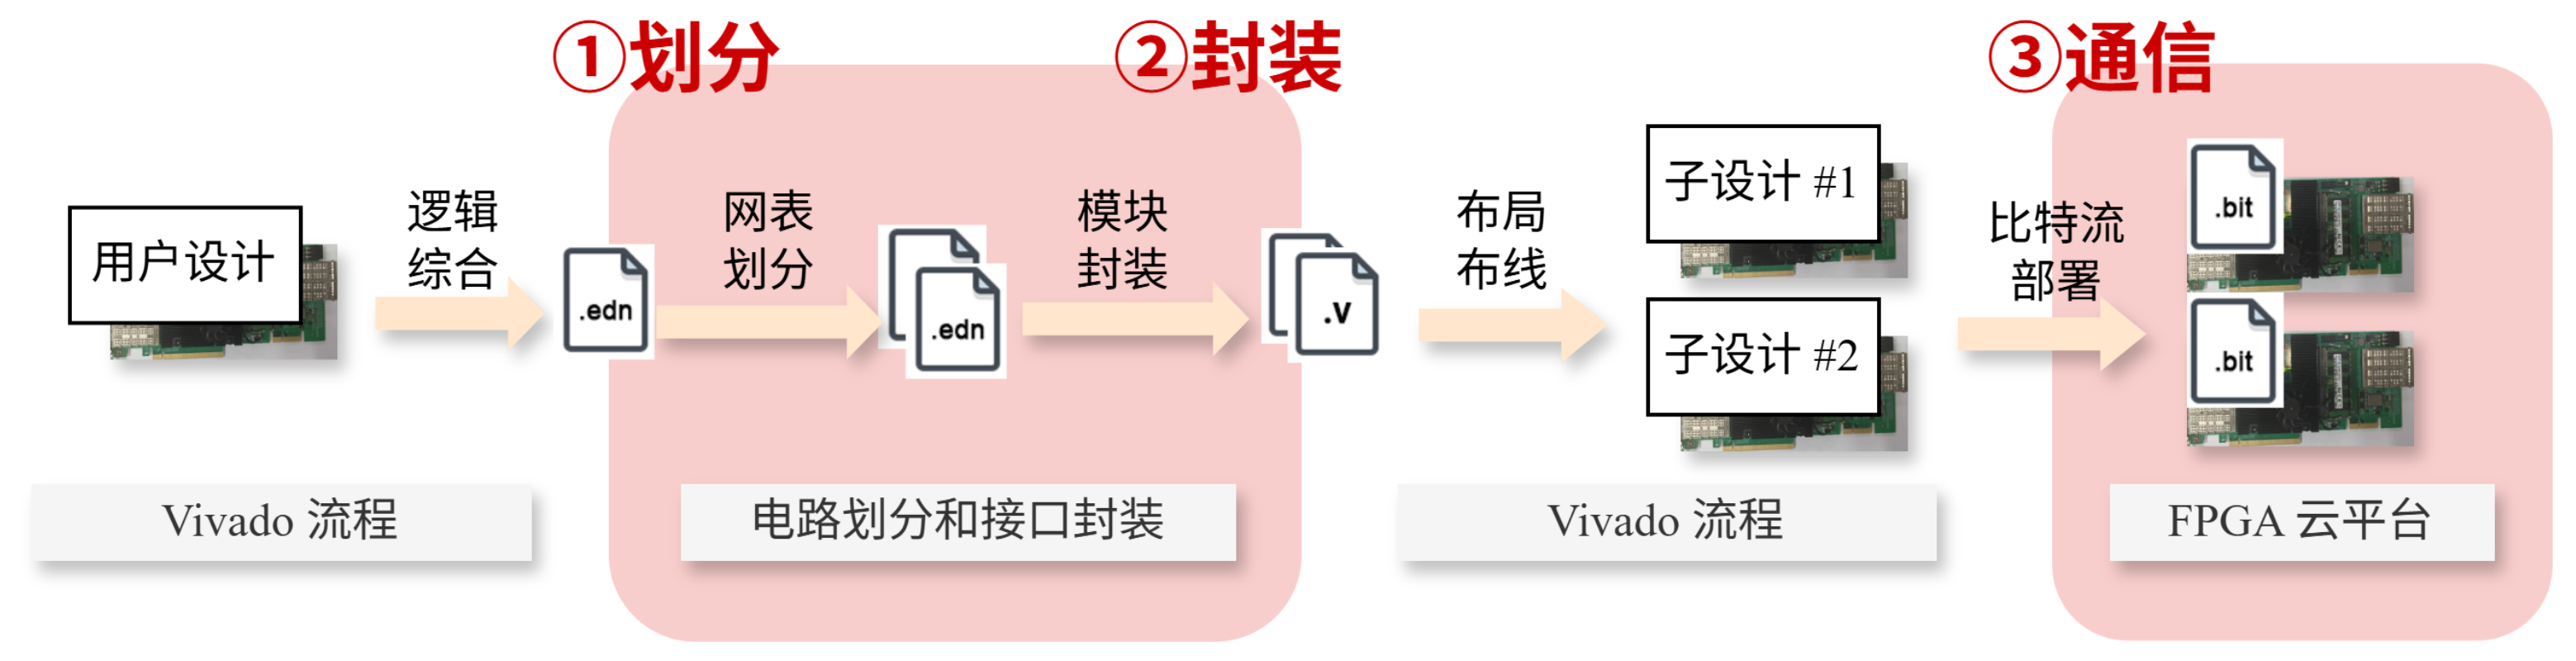
\includegraphics[width=\columnwidth]{figure/duohuafen-framework.png}
    \bicaption{DUOHUAFEN框架示意图}{DUOHUAFEN framework}
    \label{fig::duohuafen-framework}
\end{figure}

图\ref{fig::duohuafen-framework}展现了DUOHUAFEN的整体框架。在划分中，DUOHUAFEN实现了兼容标准EDIF网表格式与hMETIS超图格式的划分框架，能够将网表和超图进行双向转化，进而在电路划分领域集成了学术界典型的通用超图划分算法。本项目将延续集成超图划分算法的思路，进一步实现通用RTL的模块级划分和自适应粒度的划分。并将基于EDIF格式算法实现，进一步在广泛使用的综合器Yosys上实现。在集成中，DUOHUAFEN设计了结合LI和TDM优点的LI-TDM的跨边界接口电路。详见划分跨边界接口电路部分，在此不做赘述。在互联上，DUOHUAFEN提出了基于AXI-Stream协议的流式互连通信，用于为划分逻辑提供统一的跨节点数据交换接口，屏蔽了底层物理信道的差异。然后DUOHUAFEN依然是在同构的通信信道下构建多FPGA系统，本项目将在此基础上，利用物理信道无关的流失互联通信，在异构的通信信道中实现多FPGA的硬件仿真系统。


\subsection{硬件仿真系统开发基础平台：REMU}

REMU是一个周期精确、比特精确的FPGA硬件仿真平台\cite{chen_remu_2023}。图\ref{fig::remu-framework}展示了REMU平台的使用流程：用户仅需在主机上进行操作，通过基于PCIe的DMA数据通信，向FPGA发送控制信号。FPGA上运行着被插入扫描链的设计，设计可以被外部启动或者暂停，也可以将设计中所有时序器件的状态通过扫描链导入或导出。当x86主机获取状态检查点文件后，系统完整状态将被注入软件仿真器，在用户指定时段内实现电路级确定性重放。仿真过程中重建的波形文件包含被测设计所有电路级信号，为系统调试提供全比特精度可视化支持。

\begin{figure}[htb]
    \centering
    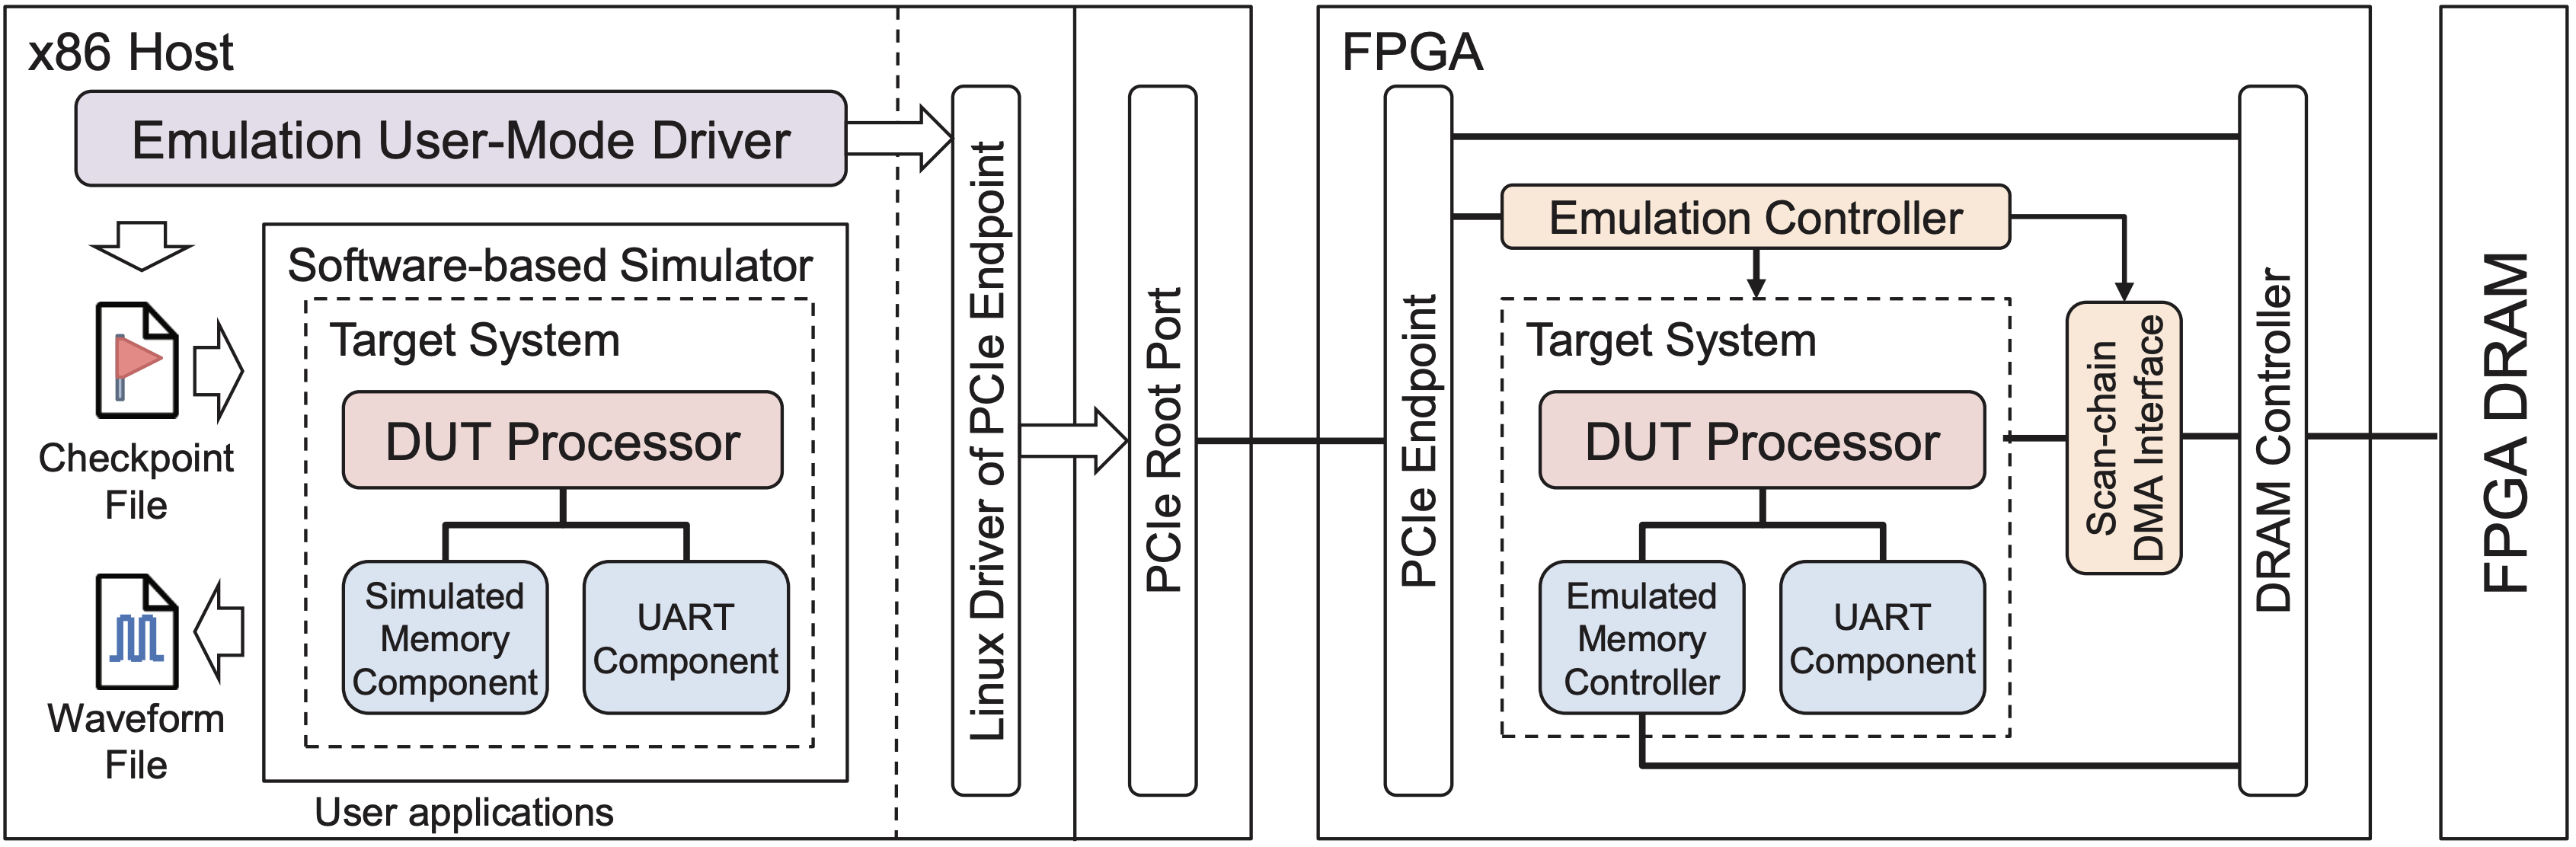
\includegraphics[width=\columnwidth]{figure/remu-framework.png}
    \bicaption{REMU硬件仿真系统整体框架}{REMU hardware emulation framework}
    \label{fig::remu-framework}
\end{figure}

为了实现全比特精确的波形重放，REMU使用了扫描链技术。扫描链的工作原理如图\ref{fig::scan-chain}所示，在开启扫描链模式的时候，时序器件的数据可以通过专用的数据通路导入或导出。相比未插入扫描链的设计，仅添加了额外的多路选择器、使能信号、以及扫描链数据通路，并未增加时序器件。扫描链是一种在不影响设计硬件电路功能的前提下，大大增加了信号可见性的方法。REMU编写了一套基于Yosys的自动化流程，用于处理时钟、插入扫描链、添加控制状态机。该课题将在原有框架下增加新的划分和集成的流程用于支持多FPGA的硬件仿真。

\begin{figure}[htb]
    \centering
    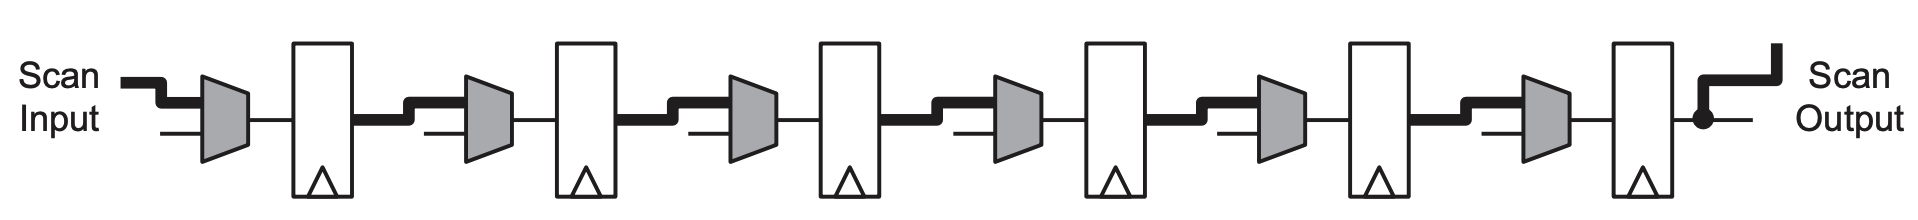
\includegraphics[width=\columnwidth]{figure/scan-chain.png}
    \bicaption{扫描链工作原理示意图}{Scan chain working principle}
    \label{fig::scan-chain}
\end{figure}


\chapter{课题研究目标、研究内容和拟解决的关键性问题}

\section{研究目标}

为填补学术界在多FPGA硬件仿真平台方面的研究空缺，本课题提出REMUS（Scalable Multi-FPGA Replayable Emulator System），一个面向多层次（片内、跨片、跨服务器）与多粒度（模块级与网表级）的多FPGA硬件仿真的开源解决方案。REMUS面向三个核心目标：可调试性、通用性、自动化。为实现这些目标，本课题在多FPGA系统部署的三大步骤——电路划分、结构集成、互联体系——中引入系统性创新，包括基于扫描链的硬件仿真技术路线、结合延迟不敏感与分时复用优势的LI-TDM跨边界接口、面向通用RTL的全自动划分与集成流程，以及基于AXI-Stream协议的流式互联通信抽象。

REMUS首先是一个周期精确、比特精确的多FPGA硬件仿真平台，能够在软件仿真环境中精确重放硬件任意周期的内部状态。其次，它提供了从RTL输入到可综合Verilog输出的全自动化流程，仅需指定划分数量即可完成完整的划分与集成，无需用户介入。再次，REMUS是一个灵活的多粒度解决方案：设计既可在模块级或网表级进行划分，也可基于资源评估动态选择合适粒度；同时支持对部分模块选择性插入扫描链以降低资源开销。最后，REMUS是跨层次通用的互联体系，支持三种部署方式：可重构区域的片内互联、点对点跨FPGA互联，以及跨服务器网络互联。

\section{关键性问题}

\begin{itemize}

    \item 电路划分：自适应粒度的全自动划分流程。实现支持自适应粒度的自动化电路划分框架，需要集成超图划分算法，并保持高度可扩展性，使设计在模块级与网表级均可进行有效分割。
          
    \item 结构集成：结合扫描链与 LI-TDM的统一集成技术。基于LI-TDM的轻量级跨边界接口与扫描链结构，对划分后的子电路进行统一集成，从而实现对内支持任意同步电路的精准划分，对外支持多种多FPGA互联架构，并为硬件仿真提供可重放的扫描链数据路径。
          
    \item 互联体系：统一可扩展的跨FPGA通信和主机通信。构建基于上述跨边界接口的多FPGA流式互联通信抽象，与物理信道解耦，可部署于片内互联、跨片点对点链路以及跨服务器网络等多层次的系统中。同时在有限的接口下构建可扩展的主机通信链路，实现一对多的控制信号和检查点数据的传输。
          
    \item 系统验证：在自建多FPGA平台上的大规模设计验证。在自主搭建的多FPGA平台上部署多种处理器或SoC的验证场景，验证所提出方法在运行性能、可扩展性与可调试性，并给出系统级评估结果。
          
\end{itemize}

\section{研究内容}

本节介绍REMUS的系统框架与设计思路。REMUS面向跨节点的多FPGA部署，旨在克服现有方案在可调试性、扩展性与自动化方面的不足。其整体流程遵循上述的多FPGA系统部署的步骤，即：电路划分、结构集成、互联体系三个核心阶段。用户只需将自定义硬件逻辑接入REMUS提供的标准化顶层接口（包括AXI存储器、串口、时钟等基础外设），无需额外修改即可进入完全自动化的处理流程。

REMUS的运行机制如图\ref{fig::remus-framework}所示：首先对输入设计执行自动化的电路划分；随后对每个划分子模块进行结构集成，包括跨FPGA数据接口与扫描链集成；最后，在多级物理架构上构建统一的通信体系，并通过运行时软件实现协同执行、暂停恢复与波形重放等能力。

\begin{figure}[htb]
    \centering
    \includegraphics[width=\columnwidth]{figure/REMUS-framework.png}
    \bicaption{REMUS框架示意图}{REMUS framework}
    \label{fig::remus-framework}
\end{figure}

\subsection{电路划分：自适应粒度的全自动划分流程}

REMUS 的第一阶段是自动化电路划分。系统基于综合工具解析并初步综合用户提供的Verilog设计，在保留层次结构的同时将内部逻辑转化为中间层原语。随后，REMUS执行划分预处理，包括模块资源评估、跨模块连线统计以及对资源占用较大的模块进行递归展开。这一预处理步骤是实现自适应粒度划分的关键，使系统能够在模块级与网表级间灵活切换，并依据资源配置自动选取合适粒度。

在此基础上，框架将预处理后的设计结构自动转换为标准化的超图表示，调用超图划分算法获得划分映射。系统在该阶段预留接口，可便捷地集成其他划分算法。最终，REMUS将划分结果写回至Verilog格式，为每个子模块插入划分属性并生成结构化的划分输出文件。划分阶段的输入与输出均保持Verilog形式，以便独立集成到其他多FPGA流程之中。

\subsection{结构集成：基于LI-TDM与扫描链的统一集成技术}

划分完成后，REMUS自动进入结构集成阶段。该阶段包含划分集成与逻辑集成两部分。

在划分集成部分，框架首先对划分产生的互联边界进行一次统一跨边界接口，将线网连接转换为协议化的数据传输接口。REMUS采用LI-TDM跨边界接口方案，它结合了延迟不敏感（Latency-Insensitive， LI）通信与分时复用（Time-Division Multiplexing， TDM）的优势，对外提供延迟不敏感接口，从而在跨FPGA通信中显著降低时序约束；对内以TDM机制驱动状态机，天然支持任意同步时序电路的划分，即便在组合逻辑存在依赖的划分边界也能避免死锁。

在逻辑集成部分，REMUS对内部所有时序器件进行统一的时钟门控改写、时钟域分析与扫描链插入，生成可精确重构电路状态的扫描链端口。然而原始扫描链控制器与LI-TDM控制器语义冲突，无法直接复用。为此，REMUS设计了新的统一控制逻辑，实现多FPGA的同步启停、扫描链双向数据传输以及周期级精确状态捕获。整个流程完全自动化，由综合工具解析划分结果并生成最终可综合的Verilog，无需用户干预。


\subsection{互联体系：统一可扩展的跨FPGA通信和主机通信}

通信阶段涉及FPGA间的运行时数据传输以及主机与FPGA间的控制通信。由于划分将电路逻辑拆解至不同FPGA，运行时中间结果无法直接送达目标寄存器，必须依赖跨FPGA通信路径进行传输。为实现通用性，REMUS为所有划分子设计提供统一的数据互联接口，使其与具体物理信道解耦。

基于多FPGA系统中对可靠数据包与动态路由的需求，REMUS采用AXI-Stream协议构建抽象化的流式互联接口，并在片内互联、跨片链路以及跨服务器网络三种架构中实现同样的通信语义，展示其多层次通用性。

另一方面，作为周期精确的硬件仿真系统，REMUS还需支持软件侧对FPGA的统一启停控制、检查点传输与波形重放。单片系统REMU采用PCIe + DMA的直接主机通信方式，但扩展至多FPGA后面临主机接口数量受限与多片消息同步的问题。为此，REMUS引入分层控制路径，通过复用FPGA间现有物理链路减少主机直接通信需求，并依靠分布式集成逻辑实现多片间同步推进。

\subsection{方法优势与对比分析}

表~\ref{tab:compare}所示，REMUS在可调试性、通用性与自动化程度上，与现有学术系统相比，均有显著提升。其自动化划分流程支持可变粒度甚至自适应粒度选择，而FireAxe在划分阶段仍需手动指导，Hetero-ViTAL仅支持模块级粗粒度划分，DUOHUAFEN仅支持网表级划分。在集成层面，REMUS是首个将扫描链与划分接口统一化的方案，实现统一的启停控制；其划分集成基于LI-TDM，既支持任意同步时序电路，又向外提供延迟不敏感接口，适用于同步与异步多FPGA系统。相比之下，FireAxe的LI-BDN接口控制逻辑复杂，而Hetero-ViTAL的LI通道限制较强，无法应用于任意电路的划分。在通信体系上，REMUS提供物理信道无关的流式互联协议，可适应异构链路结构；而Hetero-ViTAL依赖特定云平台，DUOHUAFEN与FireAxe均基于同构通信结构，通用性有限。

\begin{table}[htb]
    \centering
    \caption{REMUS与相关工作的功能对比}
    \label{tab:compare}
    \begin{tabular}{*{6}{c}}
        \toprule
        框架名称  & FireAxe & Hetero-ViTAL & DUOHUAFEN & REMU   & REMUS  \\
        \midrule
        划分粒度  & 网表      & 模块           & 网表        & -      & 网表或模块  \\
        自动划分  & 否       & 是            & 是         & -      & 是      \\
        跨边界接口 & LI-BDN  & LI           & LI-TDM    & -      & LI-TDM \\
        硬件仿真  & 否       & 否            & 否         & 是      & 是      \\
        通信体系  & 同构通信    & 网络           & 同构通信      & PCIe直连 & 异构通信   \\
        \bottomrule
    \end{tabular}
\end{table}
\chapter{拟采取的研究方法、技术路线、实验方案及其可行性分析}

\section{研究方法与技术路线}

本节介绍通用多FPGA硬件仿真系统REMUS的研究方法与技术路线。REMUS整体技术路线同样遵循上述的多FPGA系统部署的三大步骤：电路划分、结构集成、互联体系。下文将从三大步骤的角度分别进行介绍。

\subsection{模块级抽象策略与自适应粒度电路划分框架实现}

在电路和超图建模方面，首先使用开源综合工具Yosys解析RTL，将其初步转化为Yosys的中间表示，这时后期处理的基础。下一步是关键的预处理，这是实现自适应粒度的核心。如表所示，该算法会递归地遍历模块实例化树，计算每个模块的资源使用情况，并根据预设的资源阈值决定是否展开子模块。该方式能够动态地调整划分的粒度，在使得每个模块的资源使用更加均衡的同时，加快了划分算法的运行速度，不需要展开整个设计，减小了超图划分算法的输入规模。这种自适应的粒度调整机制，使得我们的划分框架能够灵活地适应不同的电路划分需求，在效率和性能之间进行良好的折中。

完成自适应预处理后，需要将设计转化为超图并调用超图划分算法。当输入是一个网表的时候，设计中的每一个实例化都是一个标准库单元，每条连接都是1位长度。每个标准库单元被抽象成为权重相同的超图节点，连接被抽象成为权重相同的超边。对于大规模的设计，转化出来的超图也会十分庞大，这对解析器和算法都提出了性能上的挑战。但这依然存在压缩的空间，因此REMUS提出了模块级的抽象策略。对于层次结构设计，仅扫描顶层的所有实例化和连接。按照连接关系，将所有实例和所有端口转化成顶点，所有的连接抽象成一条超边。此时连接不再以位为单位，而是以线网作为单位。为了实现更好的划分平衡度和真实性，我们为每一个顶点和超边赋予权重。目前顶点的权重是基于综合工具的资源评估结果，超边的权重则是基于连接的位宽。这种赋值权重的方式能很好的适配TritonPart的超图划分算法，节点的权重类型可以是一个向量，用于描述该模块所消耗的各种资源的数目。这能够使得划分结果从不同的资源占用的角度看都足够均衡。

\subsection{集成控制器的实现与仿真就绪单元}

在REMUS的集成步骤中，需要实现划分集成与扫描链集成。划分集成采用DUOHUAFEN的LI-TDM跨FPGA边界接口，而扫描链集成采用REMU的方案。尽管是已有可用的两个方案，然而REMU的扫描链控制器与 LI-TDM 控制器语义冲突，无法直接复用。REMUS需要设计了新的统一控制逻辑，实现多FPGA的同步启停、扫描链双向数据传输以及周期级精确状态捕获。

如图\ref{fig::LI-TDM}所示，LI-TDM的控制器会根据系统时钟和数据传输桥生成一个新的时钟用于控制所有时序逻辑，保证划分子设计在计算完全部的组合逻辑后才前进一个时钟周期。扫描链的控制器则更为复杂，它会生成运行时钟和扫描时钟，两个时钟都需要连接到所有时序器件中，而它的输入是系统时钟和设计中抽取的Trace信号。Trace信号是REMU流程生成的，用于在指定监视的信号发生变化时，停止设计运行。为此，REMUS将LI-TDM的生成的运行时钟转化一个使能信号，将使能信号作为一个新的Trace信号，连接到扫描链控制器的Trace信号输入中。即可保证扫描链的控制器在计算完所有的组合逻辑后，才前进一个时钟周期。经过统一后的控制器，称作集成控制器。它对外暴露的端口和REMU的扫描链控制器一致：一个AXI-Lite Slave端口用于主机对系统运行状态进行控制，一个AXI Master端口传输扫描链的数据。经过上述处理，REMUS将一个划分设计转化成了一个可综合、可暂停、可观察、可重放的“硬件仿真就绪单元”。

\begin{figure}[htb]
    \centering
    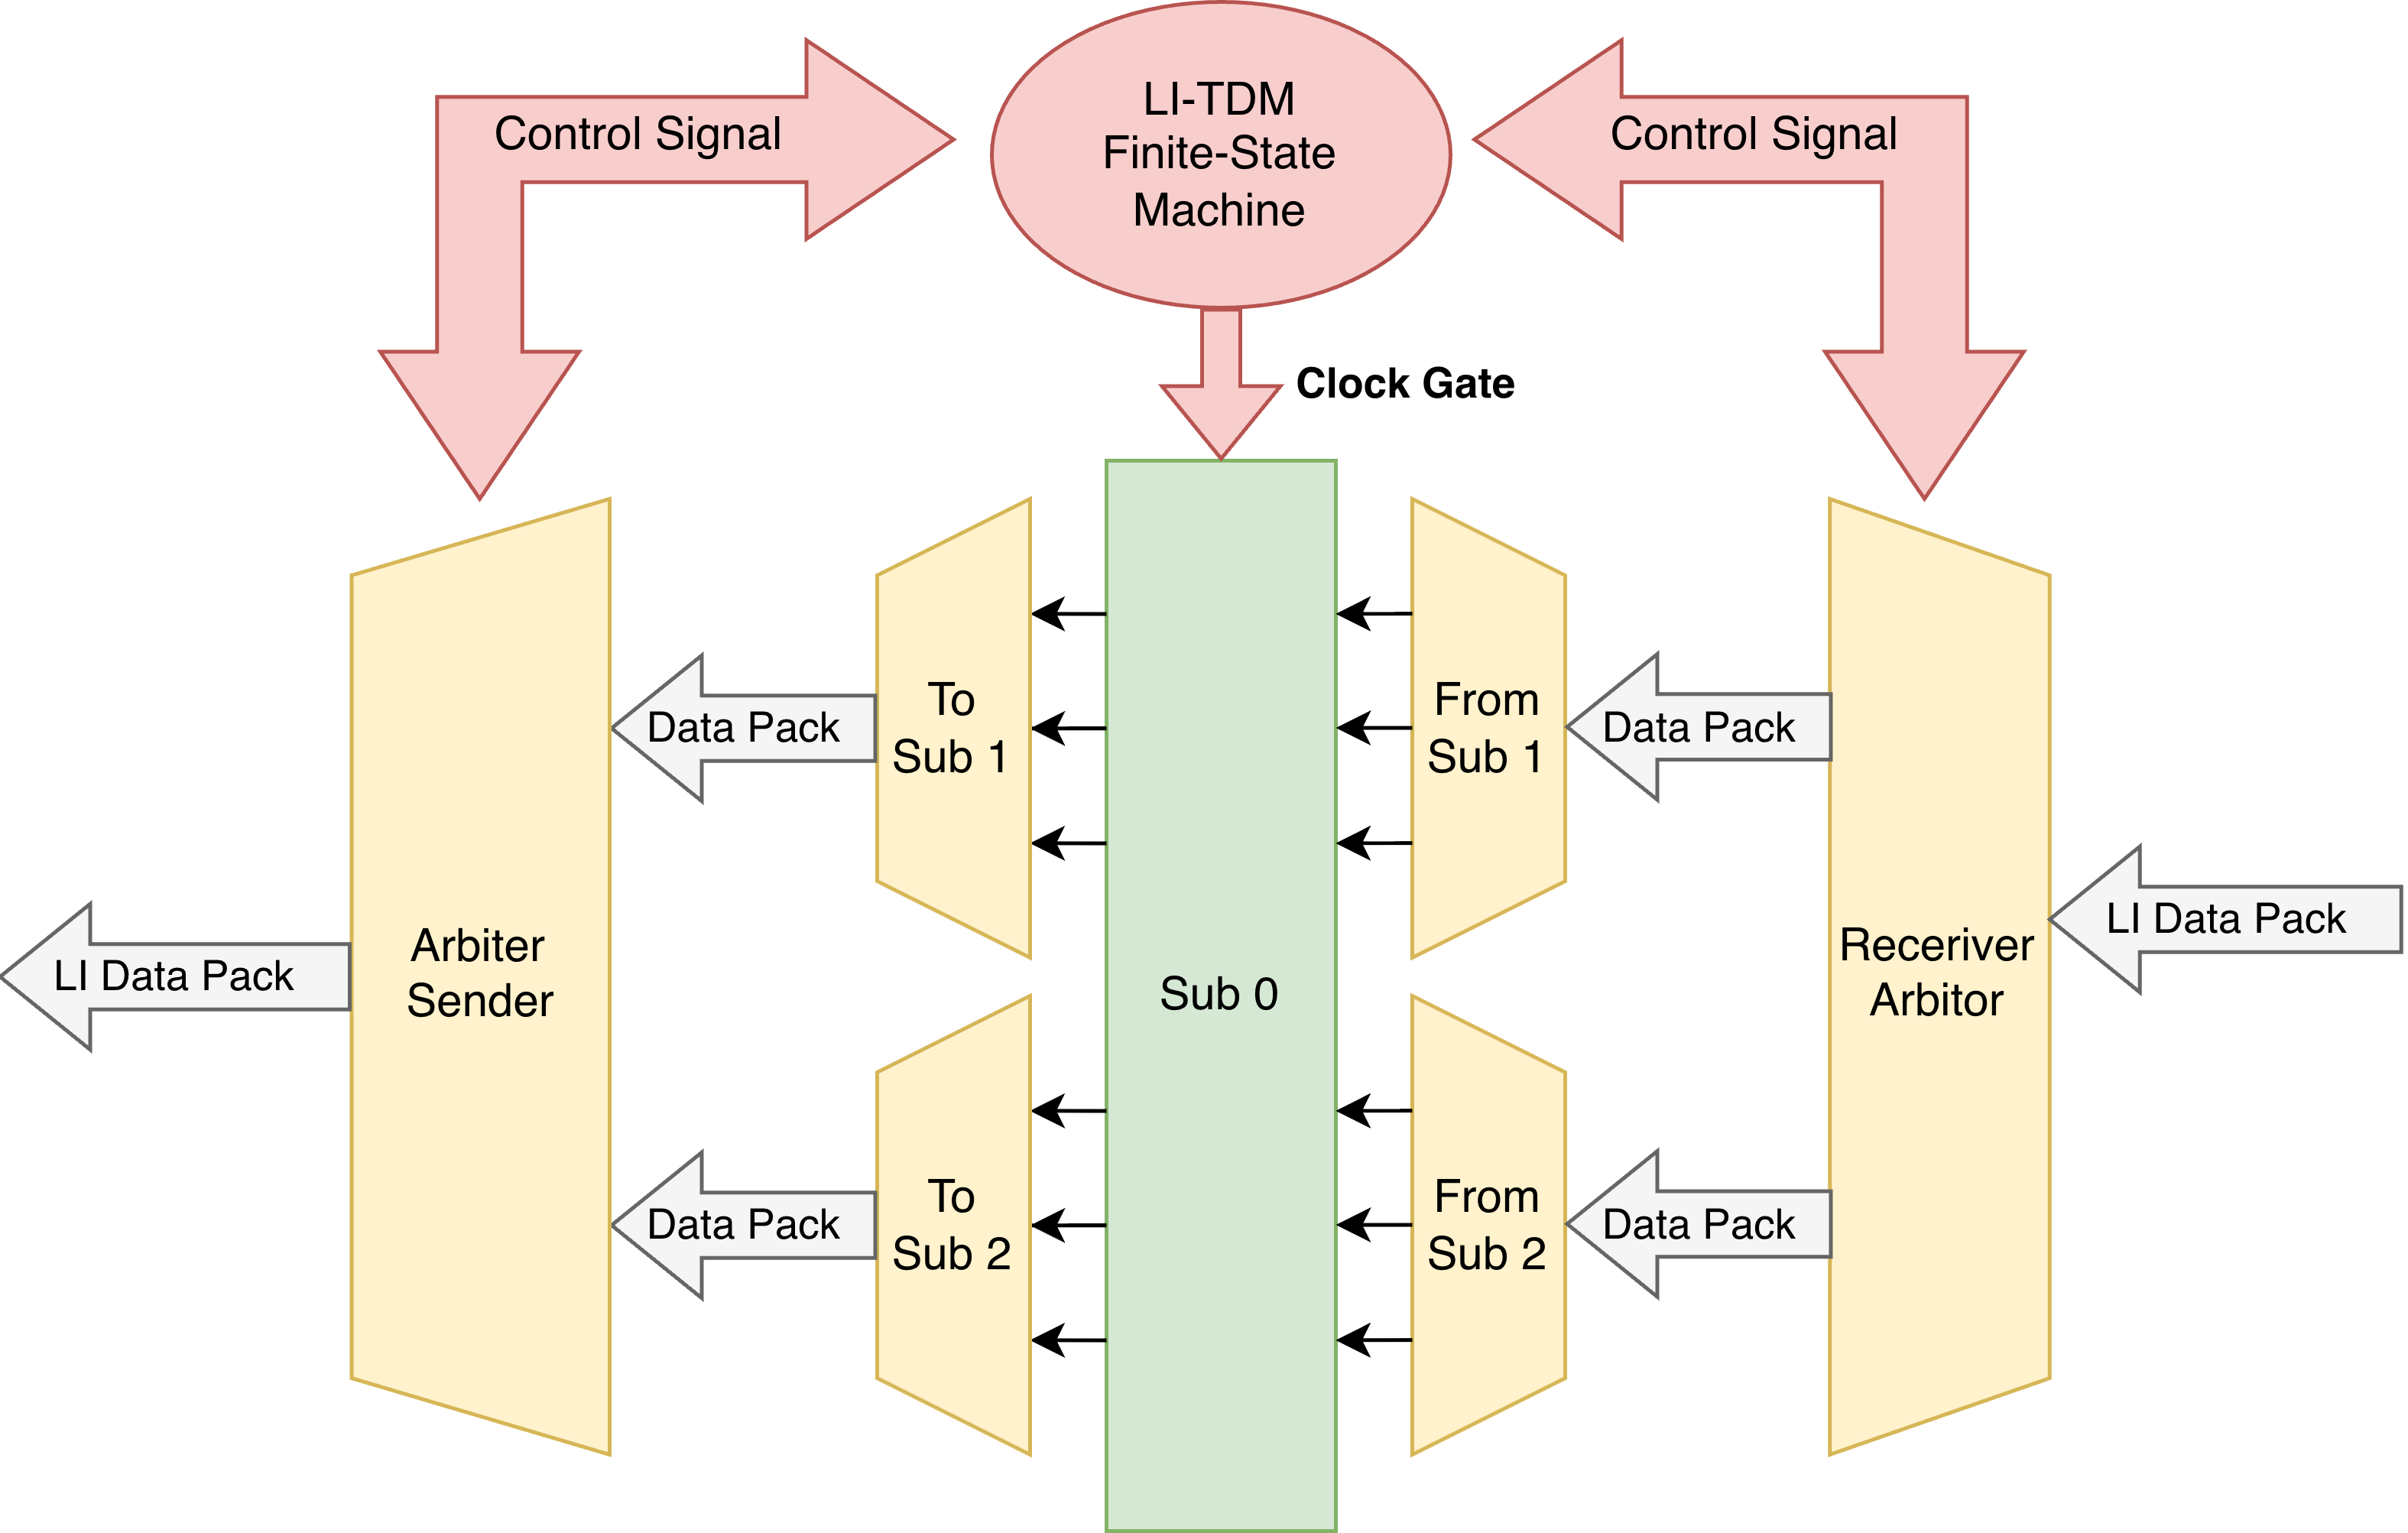
\includegraphics[width=\columnwidth]{figure/LI-TDM.png}
    \bicaption{LI-TDM跨边界接口结构}{LI-TDM cross-boundary interface structure}
    \label{fig::LI-TDM}
\end{figure}

\subsection{物理信道无关的数据平台通信与可扩展的控制平面通信}

划分和后集成，最终部署到多FPGA的计算节点上。计算节点之间互联通信，使各子模块协同工作。前文提到，我们采用AXI Stream协议来实现一种信道无关的流式互联通信。这可以帮助我们在多样化的计算节点与物理互联信道中实现统一互联，增强我们的多FPGA系统的通用性和可扩展性。

在计算节点的组织方式上，REMUS框架将计算节点视作分层架构，存在片内、跨片、和跨服务器三种层级，如图6.1所示。在片内层级，计算节点以运行时层常见的Shell-Role结构组织：每个FPGA加速卡上包含一个Shell，提供配置控制、外设接口等运行时环境，以及多个承载用户逻辑的多个Role。片间层级由多块FPGA加速卡搭配一台主机服务器组成，FPGA可能会由PCIe Switch或者QSFP光纤的方式互联。而在在片间层级，FPGA加速卡通过PCIe接口与主机相连。服务器和加速卡的组合进一步作为基本单元，形成跨服务器层级。在跨服务器层级中，FPGA加速卡和服务器主机都接入数据中心交换机。这一种往往是FPGA云服务的常见部署方式。在上述计算节点的组织架构下，两个计算节点之间存在三种基本的物理互联信道。尽管这些物理信道具有不同的传输协议和物理特性，但大都满足多FPGA系统的通信要求：以数据包形式传输，支持动态路由，具备可靠性。基于这些要求，我们可以将这些物理信道抽象为统一的AXI Stream接口，从而实现跨层级、跨信道的统一互联通信。

AXI Stream的流式互联通信，让物理信道的细节对集成控制器的通信接口透明化，从而简化了计算节点运行时环境的设计。下文介绍运行时环境为用户逻辑提供的丰富控制和通信接口，简化用户逻辑在计算节点上的部署和适配。图6.2展示了硬件逻辑部署到计算节点后的结构，该部署结构同时适用于多种互联信道。整个系统结构包括若干组件，可以分为控制平面和数据平面。数据平面用于传输FPGA跨片数据，该部分前文已经有详细的描述，在此不赘述。控制平面包括三部分：主机上运行的驱动程序、FPGA上的集成控制器、IO通信桥以及连接的相关外设。如表3.1.1所示，三个组件分工协作，在用户逻辑运行的整个周期中都发挥着重要作用。

\begin{table}[htb]
    \centering
    \caption{控制平面功能说明}
    \label{tab::control_plane}
    \begin{tabular}{*{2}{c}}
        \toprule
        运行周期 & 功能说明                        \\
        \midrule
        启动前  & 将软件负载加载到FPGA侧的内存中           \\
        启动时  & 通过扫描链将时序器件的检查点数据导出/导入       \\
        启动后  & 控制设计的启动和暂停                  \\
        启动后  & 改变DUT的输入端口的数据，观察输出端口的数据     \\
        启动后  & 通过串口控制器等外设监控计算节点的运行状态，并与之交互 \\
        \bottomrule
    \end{tabular}
\end{table}

对于发送启停信号，在单片的REMU系统中，主机程序通过PCIe向FPGA上的集成控制器发送写请求，修改内部控制状态寄存器，从而实现控制设计模式切换。在多片的REMUS中，主机驱动程序需要对所有的PCIe设备同时发送写请求，同时修改所有集成控制器的状态。虽然无法保证主机控制程序发送的写请求同时到达每一个集成控制器，但LI-TDM的的设计策略可以保证，他们一定是在完成当前周期的计算之后，才更改内部控制状态寄存器。最终实现所有的子设计全部停止在相同的周期。而对于外设相关的功能，本质上是要求主机驱动程序能够和FPGA上的外设进行交互，这往往也可以通过基于PCIe的DMA或者GPIO来实现。为了简化了外设相关的软件设计，REMUS将I/O通信接口限制在了一个计算节点，其他计算节点只需进行同步的启停操作。除了外设和主机驱动程序的交互，还需要保证外设能和划分逻辑正确的通信，REMUS的运行时环境为划分模块提供了基于AXI的外设接口。需要注意的是外设并不是直接连接到用户逻辑上，而是通过Shell中的I/O通信桥和划分逻辑通信。因为外设运行在计算节点的系统时钟下，而划分逻辑运行在由状态机控制的时钟门控下。I/O通信桥负责在两种时钟域下进行数据传输，并通过FIFO缓冲区实现跨时钟域的数据可靠传输。使得跨时钟域通信对用户逻辑透明化，简化用户逻辑的设计。

\subsection{实验方案及可行性分析}

基于前面章节所提出的研究方法和技术路线，为REMUS设计了相应的实验用于评测REMUS的功能完整性和性能。本节首先介绍多FPGA硬件仿真框架REMUS的具体部署和测试环境，然后介绍各组件的性能测试的实验设计，最后介绍一些端到端的系统试验设计。

对于划分组件的测试，运行的硬件平台是使用Xeon Gold 6338N(128)@3.50GHz处理器核的EDA服务器。划分软件是是基于开源综合工具Yosys 0.52开发的。使用标准的Titian32标准划分数据集以及三个RISC-V开源处理器进行划分实验。评价指标包括切割的组合逻辑数、跳数，以及程序的运行时间。Baseline采用使用相同的超图划分算法KaHyPar、DUOHUAFEN的划分组件，并对比了不同的划分粒度下的划分结果。为了确保划分结果的功能正确性，还会使用形式化验证和逻辑仿真两种方法，测试划分结果没有改变设计的逻辑功能。这种动静结合的测试方法，不光能够有效地发现划分过程中可能引入的错误，还能够快速精确的定位出错现场。加快调试速度，从而确保划分算法正确无误地实现。

集成组件的实验在同样的EDA服务器上进行，使用的FPGA工具链为Xilinx/Vivado2020.2。实验会在相同的划分结果下，对比LI-BDN、LI- TDM跨边界接口电路、REMU扫描链控制单元、REMUS集成控制器的接口电路资源占用和关键路径时序。而在正确性方面，逻辑仿真软件同样是一个重要的保证。首先，需要搭建一个专门多FPGA系统的仿真环境。该仿真环境使用进程间通信来模拟的FPGA之间的数据交换通路，实现跨片数据的传输。使用内存文件映射来模拟PCIe设备在主机通讯节点，实现主机驱动程序和FPGA之间的控制通路。完备的逻辑仿真可以尽可能减少上板时出现的异常情况，提高项目的可行性。

对于通信实验，计划部署了如下的异构FPGA系统：使用多张课题组内自建的FPAG板卡——NewMemory，基于VU37P FPGA芯片。测试和评估在一台主机服务器内，通过PCIe物理信道使两个FPGA芯片上的计算节点协同工作。在具体的组织形式上，两张加速卡搭配一台主机服务器，通过PCIex16接口将加速卡与服务器连接。跨片数据通过主机进行转发。我们还实现了基于QSFP或高速以太网物理信道的跨节点通信。

最后，本项目计划搭建一个多FPGA和x86主机的松耦合异构计算平台，预计最终实现4个FPGA和一台主机的互联。该平台上会部署了多个RISC-V处理器核，运行相同benchmark，对比了不同物理信道和时钟频率下的逻辑时钟频率和运行裸机程序的性能。
\chapter{计划进度和预期成果}

本项目预计在中期前完成所有组件的开发和测试工作，并搭建双板的一个小型的多FPGA硬件仿真系统进行初步的测试和评估。中期后会进行规模扩大和性能调优，编写毕业论文等相关事宜。具体时间安排如图~\ref{fig:project_timeline}所示：

\begin{figure}[htb]
    \centering
    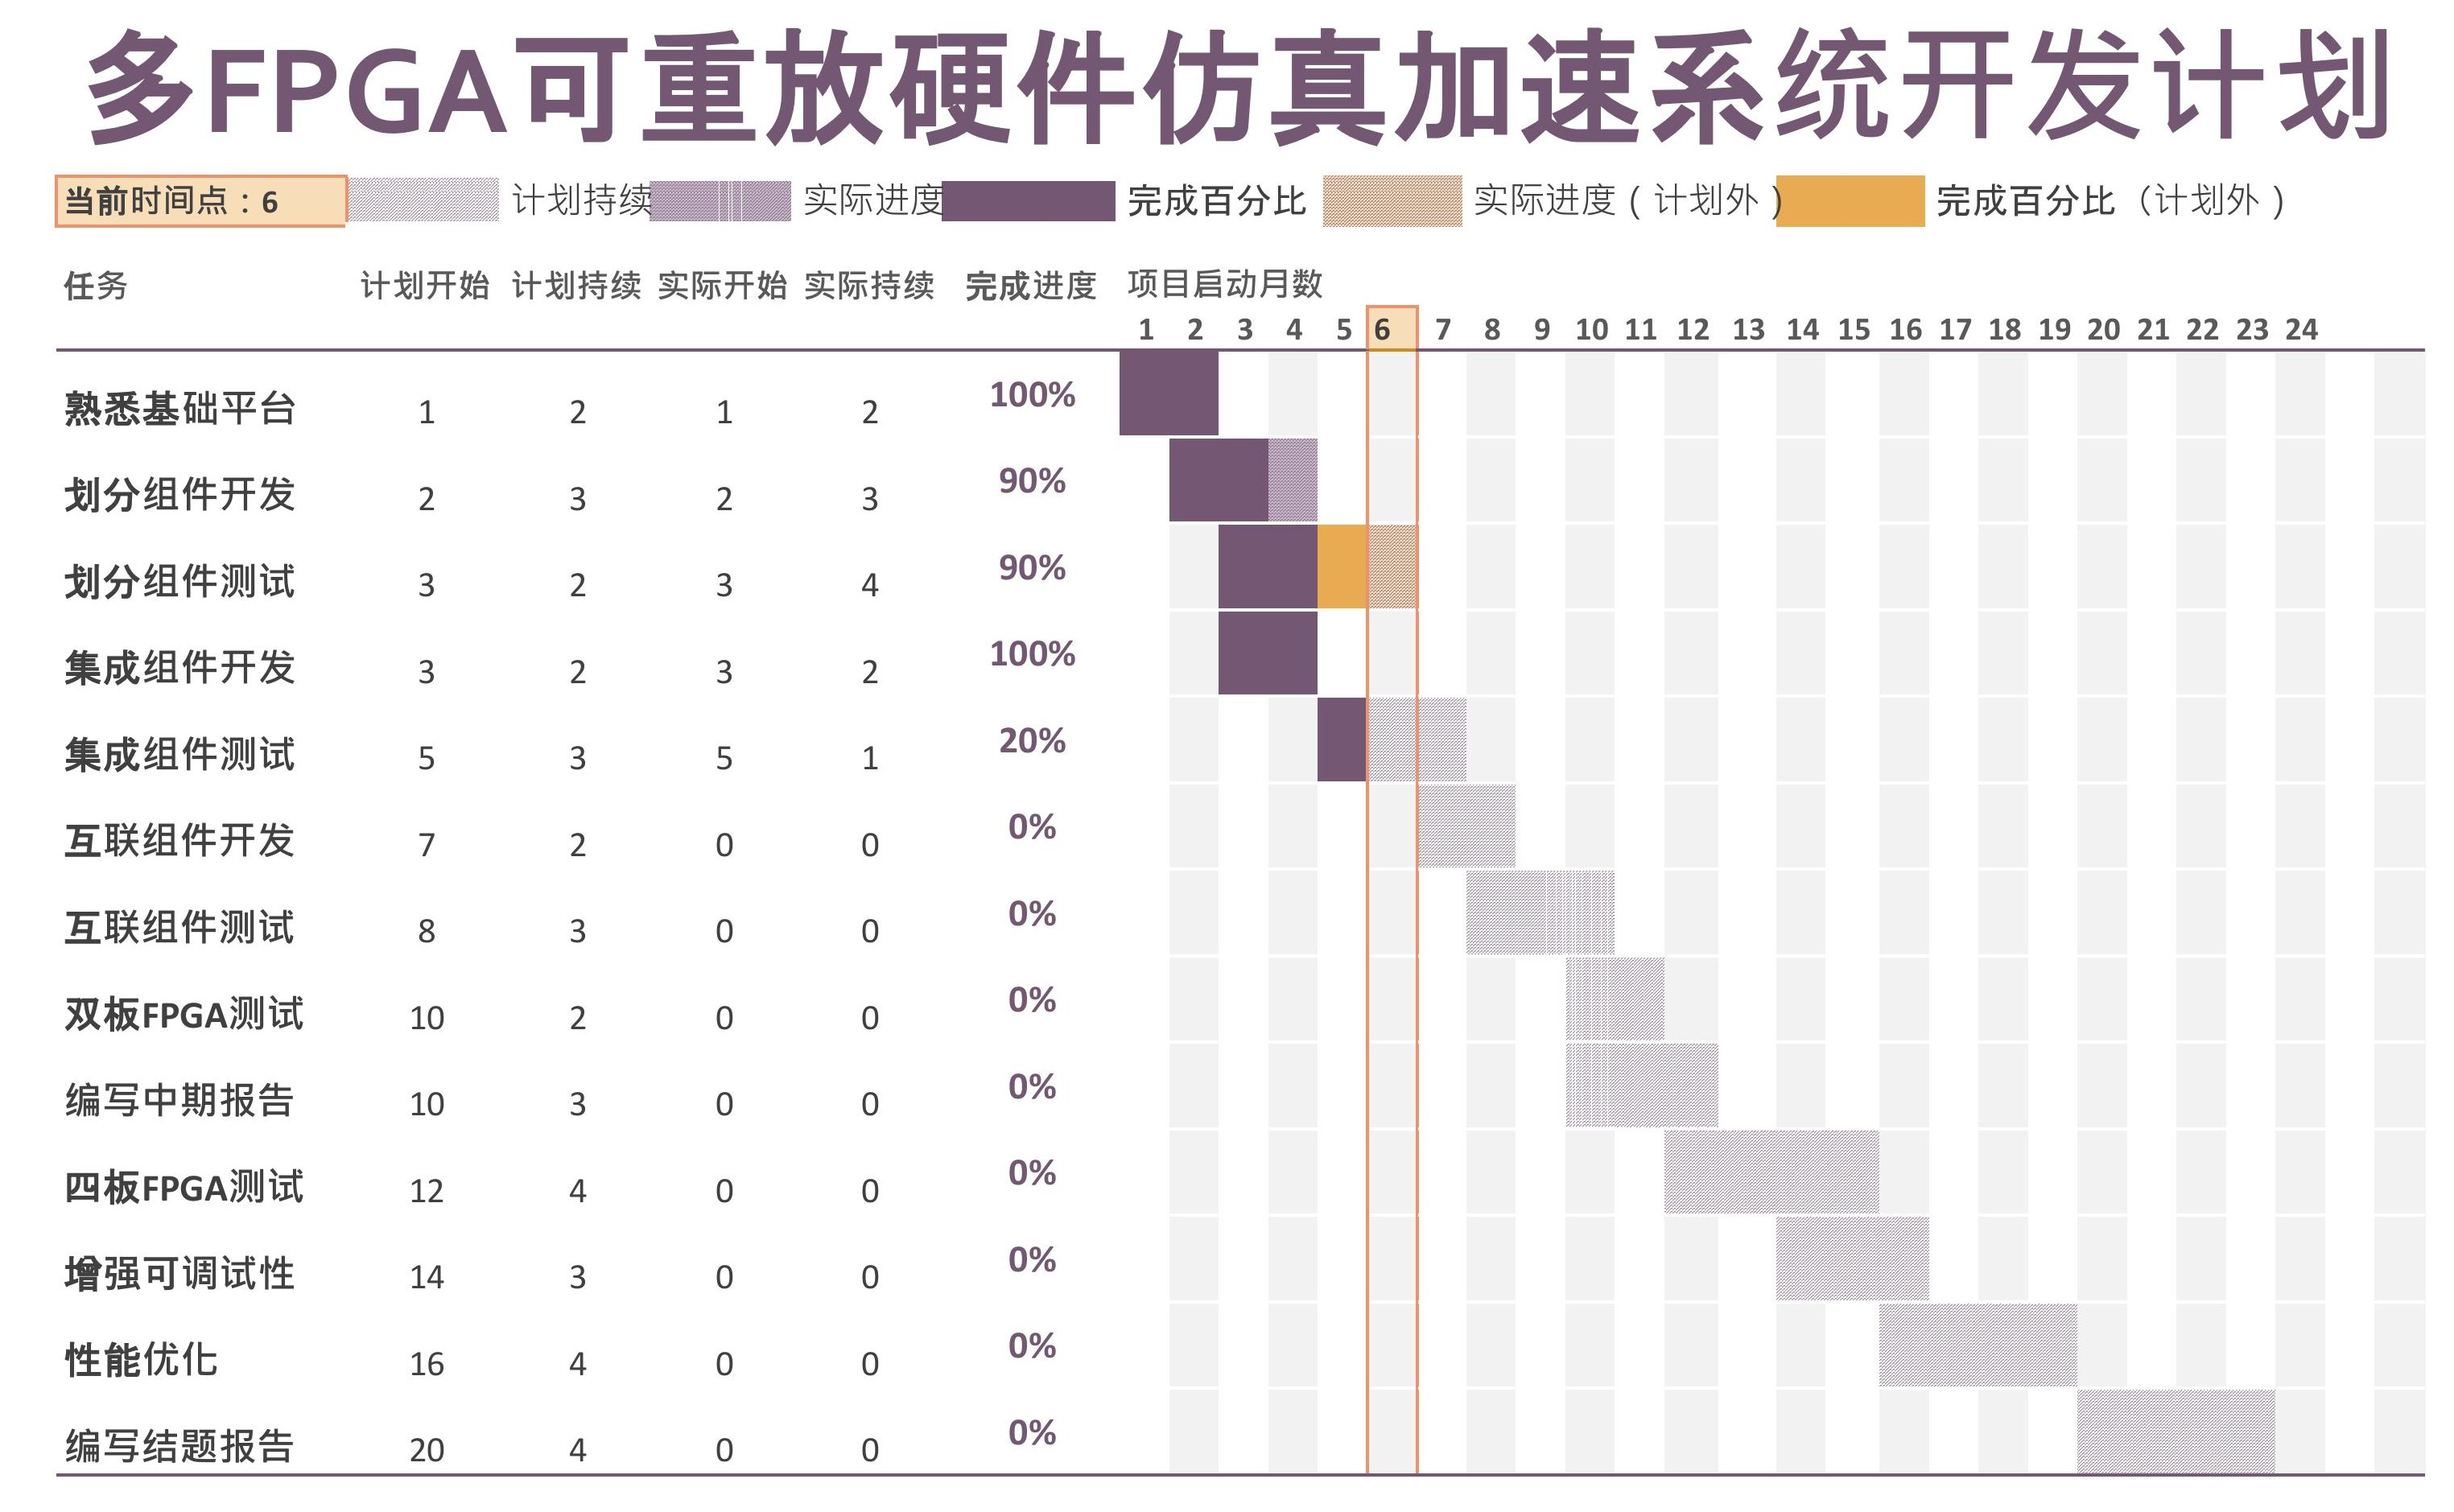
\includegraphics[width=\columnwidth]{figure/plan.jpg}
    \bicaption{项目计划时间表}{Project Timeline}
    \label{fig:project_timeline}
\end{figure}

目前已经完成了划分组件的开发和测试、跨边界接口组件的开发、互连组件的开发。预计在中期，得到一个可以稳定运行的2个FPGA硬件仿真系统，系统上部署了Picorv32为CPU的小型SoC，处理器运行裸机程序，能够实现暂停、波形重放等主要的调试功能。在结题阶段，展示一个可以5MHz运行的4个FPGA的硬件仿真系统，部署一个四核的香山昆明湖处理器和相应外设，支持波形重放、Trace等全部调试功能，能够运行并调试操作系统和应用程序。


\makebiblio

\end{document}
